%!TeX spellcheck=en_US
\documentclass[11pt,
               a4paper,
               bibtotoc,
               idxtotoc,
               headsepline,
               footsepline,
               footexclude,
               BCOR12mm,
               DIV13,
               openany,   % using this removes blank pages around part / chapter starts.
%               oneside    % include this if you have to print only one page per sheet of paper.
               ]
               {scrbook}

%%% SETTINGS

% no word wrapping
%\righthyphenmin=62
%\lefthyphenmin=62
% fewer hyphens
\usepackage{microtype}

% german symbols
\usepackage[utf8]{inputenc}

% strikethrough by \sout
\usepackage[normalem]{ulem}

% insert graphics
\usepackage{graphicx}
% more flexible figures e.g. graphics with captions beside them
\usepackage{floatrow}
% more flexible captions.
% Use \captionsetup{options} to configure,
% use it in an environment for local setup
\usepackage{caption}
% subfigures (see template):
\usepackage{subcaption}

% more control of enumerations and itemizations
\usepackage{enumitem}
% less space between items
\setlist[itemize]{itemsep=0cm}
\setlist[enumerate]{itemsep=0cm}
% more customizeable tables (e.g. multiple lines per cell)
\usepackage{tabularx}
% fix for vertical centering
\usepackage{ragged2e}
\renewcommand\tabularxcolumn[1]{>{\Centering}m{#1}}
% column types with multiple lines and formatting
\usepackage{array}
\newcolumntype{C}{>{\centering\arraybackslash}X}
\newcolumntype{R}{>{\raggedleft\arraybackslash}X}
\newcolumntype{L}{>{\raggedright\arraybackslash}X}
% merge multiple rows \multirow{2}{*}{bla} & \\ &
\usepackage{multirow}
% activate for tables with page breaking
%\usepackage{ltablex}
% fix for table movement and itemizations
%\keepXColumns

% fix for dynamics spaces after custom commands
\usepackage{xspace}

% tabbing: use with \tab
\usepackage{tabto}
\TabPositions{4cm}

%% fancy math
% propper matrices, underbrace text
%\usepackage{amsmath}
\usepackage{mathtools}
% special symbols e.g. squares
\usepackage{amssymb}

%% plotting
\usepackage{pgfplots}
\usepgfplotslibrary{fillbetween}

%%Settings for code
% code placement right there
\usepackage{float}
% code coloring
\usepackage{xcolor}
% code listing
\usepackage{listings}

% flexible multi column style
\usepackage{multicol}

% graphs
\usepackage{tikz}
\usetikzlibrary{shapes.geometric, arrows}
% define some elements
\tikzstyle{startstop} = [rectangle, rounded corners, minimum width=3cm, minimum height=1cm,text centered, draw=black, fill=blue!30]
\tikzstyle{arrow} = [thick,->,>=stealth]

% Some code highlighting styles you can use with lstlistings
% C++ code style similar to default eclipse
\lstdefinestyle{eclipse-cpp} {
    captionpos=bottom,
    language=C++,
    otherkeywords={final},
    basicstyle=\footnotesize,
    numbers=left,
    numberstyle=\small,
    showstringspaces=false,
    tabsize=2,
    frame=single,
    breaklines=true,
    keywordstyle=\bfseries\color[RGB]{127,0,85},
    identifierstyle=\color[RGB]{0,0,192},
    stringstyle=\color[RGB]{42,0,255},
    commentstyle=\color[RGB]{63,127,95},
}

% If no highlighting is intended
\lstdefinestyle{plain}{
}

% fancy algorithms (see template)
\usepackage[ruled, vlined, linesnumbered]{algorithm2e}
\DontPrintSemicolon
\SetKw{KwBy}{by}
\SetKw{KwAnd}{and}

% clickable links and clickable table of content <3
% Options: links with linebreaks
\PassOptionsToPackage{hyphens}{url}\usepackage[bookmarks=false]{hyperref}
\hypersetup{
    colorlinks,
    citecolor=black,
    filecolor=black,
    linkcolor=black,
    urlcolor=black
}
% Alterations to labels used by \autoref{}: Capitalize everyything
\def\chapterautorefname{Chapter}
\def\sectionautorefname{Section}
\def\subsectionautorefname{Subsection}
\def\algorithmautorefname{Algorithm}
\def\subfigureautorefname{Figure}
% for custon stuff like use:
% \hyperref[custom:foo]{Custom~\ref*{custom:foo}}


\usepackage{lipsum} % for filling pages with stuff

% -------------------------------------------------------------------------------
% --------------------------------- Thesis Info ---------------------------------
% -------------------------------------------------------------------------------

% set title, authors and stuff for the cover
% docytype needs xspace because it is used within text.
\def\doctype{Bachelor's Thesis\xspace}
\def\studyProgram{Informatics}
\def\title{Efficient Trajectory Modelling for Space Debris Evolution}
% don't try translate every technical term if it would sound off
\def\titleGer{Effiziente Modellierung zur Vorausberechnung von Weltraumschrott Flugbahnen}
\def\author{Oliver Bösing}
% Prof
\def\supervisor{Univ.-Prof. Dr. Hans-Joachim Bungartz}
% PhD Candidate
\def\advisor{Fabio Alexander Gratl, M.Sc.}
\def\date{15.09.2021}

\begin{document}
\frontmatter
% -------------------------------------------------------------------------------
% ---------------------------------- COVERPAGE ----------------------------------
% -------------------------------------------------------------------------------

% correct BCOR - undo at the end !!!
\def\bcorcor{0.15cm}
\addtolength{\hoffset}{\bcorcor}
\thispagestyle{empty}
\vspace{4cm}
\begin{center}
    
\includegraphics[width=4cm]{templateStuff/tumlogo.pdf}\\[5mm]
    \huge FAKULTÄT FÜR INFORMATIK\\[5mm]
    \large DER TECHNISCHEN UNIVERSITÄT MÜNCHEN\\[24mm]

    {\Large \doctype in \studyProgram}\\[20mm]
    {\huge\bf \title\par}
    \vspace{15mm}
    {\LARGE  \author}
    \vspace{10mm}
    \begin{figure}[h!]
        \centering
        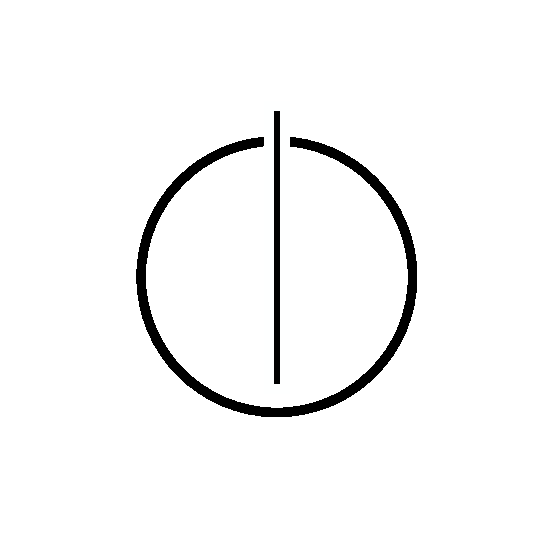
\includegraphics[width=4cm]{templateStuff/informat.pdf}
   \end{figure}
\end{center}

\cleardoubleemptypage

% -------------------------------------------------------------------------------
% ---------------------------------- TITLEPAGE ----------------------------------
% -------------------------------------------------------------------------------

\def\bcorcor{0.15cm}
\addtolength{\hoffset}{\bcorcor}
\thispagestyle{empty}
\vspace{10mm}
\begin{center}
    
\includegraphics[width=4cm]{templateStuff/tumlogo.pdf}\\[5mm]
	\huge FAKULTÄT FÜR INFORMATIK\\[5mm]
	\large DER TECHNISCHEN UNIVERSITÄT MÜNCHEN\\[24mm]
	{\Large \doctype in \studyProgram}\\[20mm]
	{\LARGE\bf \title}\\[10mm]
	{\LARGE\bf \titleGer}\\[10mm]
	\begin{tabular}{ll}
		\Large Author:      	& \Large \author \\[2mm]
		\Large Supervisor:  	& \Large \supervisor\\[2mm]
		\Large Advisor:			& \Large \advisor\\[2mm]
		\Large Date:       		& \Large \date
	\end{tabular}
	\vspace{-1mm}
	\begin{figure}[h!]
		\centering
		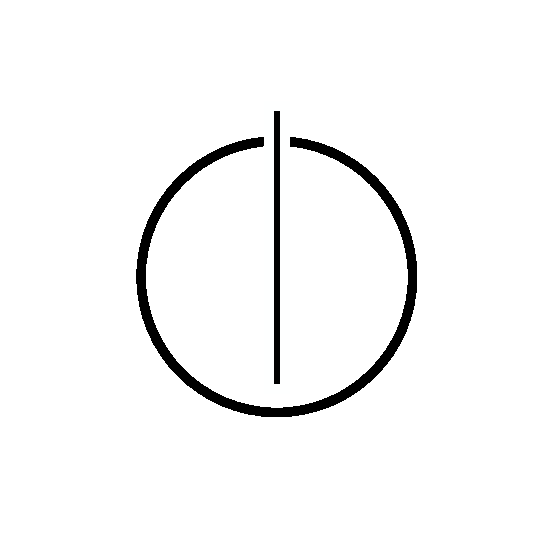
\includegraphics[width=4cm]{templateStuff/informat.pdf}
	\end{figure}
\end{center}

% undo BCOR correction
\addtolength{\hoffset}{\bcorcor}
\newpage

% -------------------------------------------------------------------------------
% ---------------------------------- DISCLAIMER ---------------------------------
% -------------------------------------------------------------------------------

\cleardoubleemptypage

\thispagestyle{empty}
\vspace*{0.7\textheight}
\noindent
I confirm that this \MakeLowercase{\doctype} is my own work and I have documented all sources and material used.\\

\vspace{15mm}
\noindent
Munich, \date \hspace{5cm} \author
\cleardoubleemptypage

% -------------------------------------------------------------------------------
% ------------------------------- ACKNOWLEDGEMENTS ------------------------------
% -------------------------------------------------------------------------------

\phantomsection
\addcontentsline{toc}{chapter}{Acknowledgements}
\vspace*{2cm}
\begin{center}
    {\Large \bf Acknowledgements}
\end{center}
\vspace{1cm}


\cleardoublepage

% -------------------------------------------------------------------------------
% ---------------------------------- ABSTRACT -----------------------------------
% -------------------------------------------------------------------------------

\phantomsection
\addcontentsline{toc}{chapter}{Abstract}
\vspace*{2cm}
\begin{center}
    {\Large \bf Abstract}
\end{center}
\vspace{1cm}


\cleardoublepage

\phantomsection
\addcontentsline{toc}{chapter}{Zusammenfassung}
\vspace*{2cm}
\begin{center}
    {\Large \bf Zusammenfassung}
\end{center}
\vspace{1cm}

\lipsum[2]

\cleardoublepage

% -------------------------------------------------------------------------------
% ------------------------------ TABLE OF CONTENTS ------------------------------
% -------------------------------------------------------------------------------

\tableofcontents
\thispagestyle{empty}
\cleardoubleemptypage

% -------------------------------------------------------------------------------
% --------------------------------- MAIN MATTER ---------------------------------
% -------------------------------------------------------------------------------

\mainmatter
\part{Abstract}
    \begin{itemize}
        \item
        \item
        \item
    \end{itemize}

\part{Introduction and Background}
\chapter{Introduction}
    \begin{itemize}
        \item Projects like Starlink, Kuiper Project, Guowang etc. plan to launch thousands of satellites in the next years
        \item with the number of satellites the number of possible collisions grow rapidly
        \item Collision events create great amounts of debris, possibly triggering a chain reaction of consecutive collisions
        \item Rising number of both, satellites and space debris, in orbits around earth lead to the need for modelling their trajectories, to predict possible collisions and act in advance to avoid them.
        \item Aim of this Thesis is to develop a software solution, to model the trajectories of particles in relevant satellite orbits, to be used by the ESA for their evolution simulation
    \end{itemize}

\chapter{Theoretical background}
\section{Equations of motion}
    \begin{itemize}
        \item the used Reference frame of the model is the EME2000 fixed frame
        \item The Motion of a particle in the used model is defined by a system of differential equations representing 8 accelerations acting on the particle
        \begin{equation}
            \begin{array}{ll}
                 \ddot{X} = f_{Kep,X}(X,Y,Z)+f_{J2,X}(X,Y,Z)+f_{C22,X}(X,Y,Z,t)+f_{S22,X}(X,Y,Z,t)\\
                +f_{Moon,X}(X,Y,Z,t)+f_{Sun,X}(X,Y,Z,t)+f_{SRP,X}(X,Y,Z,AOM)+f_{Drag,X}(X,Y,Z,A,m,v) \\
                \ddot{Y} = f_{Kep,Y}(X,Y,Z)+f_{J2,Y}(X,Y,Z)+f_{C22,Y}(X,Y,Z,t)+f_{S22,Y}(X,Y,Z,t)\\
                +f_{Moon,Y}(X,Y,Z,t)+f_{Sun,Y}(X,Y,Z,t)+f_{SRP,Y}(X,Y,Z,AOM)+f_{Drag,Y}(X,Y,Z,A,m,v) \\
                \ddot{Z} = f_{Kep,Z}(X,Y,Z)+f_{J2,Z}(X,Y,Z)+f_{C22,Z}(X,Y,Z,t)+f_{S22,Z}(X,Y,Z,t)\\
                +f_{Moon,Z}(X,Y,Z,t)+f_{Sun,Z}(X,Y,Z,t)+f_{SRP,Z}(X,Y,Z,AOM)+f_{Drag,Z}(X,Y,Z,A,m,v)
            \end{array}
        \end{equation}

        \item Kepler: two body system calculates the acceleration acting on the particle due to gravitation, assuming two point masses
        \begin{equation}
            \begin{array}{ll}
                f_{Kep,X}(X,Y,Z) &= -{GM_E X\over (X^2+Y^2+Z^2)^{3/2}}\\
                f_{Kep,Y}(X,Y,Z) &= -{GM_E Y\over (X^2+Y^2+Z^2)^{3/2}}\\
                f_{Kep,Z}(X,Y,Z) &= -{GM_E Z\over (X^2+Y^2+Z^2)^{3/2}}
            \end{array}
        \end{equation}
        \item Third body perturbations: Additional gravitational acceleration is inflicted on a particle by other bodies.
        The use model takes into account two bodies in addition to the earth. Resulting in similar Equations for this two components.
        \item Solar tide: Due to the great distance between the sun and the earth the position calculations used in the model are derived from the earths,
        i.e. the origin of our reference frame, trajectory around the sun.
        \begin{equation}
            \begin{array}{ll}
                f_{Sun,X}(X,Y,Z,t) &=-G M_\odot\left(
                {(X-X_\odot)\over [(X-X_\odot)^2+(Y-Y_\odot)^2+(Z-Z_\odot)^2]^{3/2}}
                +{X_\odot\over(X_\odot^2+Y_\odot^2+Z_\odot^2)^{3/2}} \right)\\
                f_{Sun,Y}(X,Y,Z,t) &=-G M_\odot\left(
                {(Y-Y_\odot)\over [(X-X_\odot)^2+(Y-Y_\odot)^2+(Z-Z_\odot)^2]^{3/2}}
                +{Y_\odot\over(X_\odot^2+Y_\odot^2+Z_\odot^2)^{3/2}} \right)\\
                f_{Sun,Z}(X,Y,Z,t) &=-G M_\odot\left(
                {(Z-Z_\odot)\over [(X-X_\odot)^2+(Y-Y_\odot)^2+(Z-Z_\odot)^2]^{3/2}}
                +{Z_\odot\over(X_\odot^2+Y_\odot^2+Z_\odot^2)^{3/2}} \right)
            \end{array}
        \end{equation}
        where
        \begin{equation}
            \begin{pmatrix}
                X_\odot\\
                Y_\odot\\
                Z_\odot
            \end{pmatrix} =
            \begin{pmatrix}
                r_\odot \cos \lambda_\odot\\
                r_\odot \sin \lambda_\odot \cos \varepsilon\\
                r_\odot \sin \lambda_\odot \sin \varepsilon
            \end{pmatrix}
        \end{equation}
        with
        \begin{equation}
            \begin{array}{ll}
                \lambda_\odot &= \Omega_\odot+\omega_\odot+\ell_{\odot}+\left(
                {6892\over3600} \sin \ell_{\odot} + {72\over 3600} \sin 2\ell_{\odot}\right)\\
                r_\odot[10^6\mbox{km}] &=149.619-2.499 \cos \ell_{\odot} - 0.021 \cos 2\ell_{\odot}\\
                \ell_{\odot} &= \varphi_{\odot,0}+\nu_\odot t
            \end{array}
        \end{equation}
        \item Lunar Tide: Because the Moon is significantly closer to the earth than the sun the calculations of its position is done with a higher accuracy than for the calculation of the suns position.
        \begin{equation}
            \begin{array}{ll}
                f_{Moon,X}(X,Y,Z,t) &=-G M_{\mathcal M}\left({(X-X_{\mathcal M})\over [(X-X_{\mathcal M})^2+(Y-Y_{\mathcal M})^2+(Z-Z_{\mathcal M})^2]^{3/2}}
                +{X_{\mathcal M}\over(X_{\mathcal M}^2+Y_{\mathcal M}^2+Z_{\mathcal M}^2)^{3/2}} \right)\\
                f_{Moon,Y}(X,Y,Z,t) &=-G M_{\mathcal M}\left({(Y-Y_{\mathcal M})\over [(X-X_{\mathcal M})^2+(Y-Y_{\mathcal M})^2+(Z-Z_{\mathcal M})^2]^{3/2}}
                +{Y_{\mathcal M}\over(X_{\mathcal M}^2+Y_{\mathcal M}^2+Z_{\mathcal M}^2)^{3/2}} \right)\\
                f_{Moon,Z}(X,Y,Z,t) &=-G M_{\mathcal M}\left({(Z-Z_{\mathcal M})\over [(X-X_{\mathcal M})^2+(Y-Y_{\mathcal M})^2+(Z-Z_{\mathcal M})^2]^{3/2}}
                +{Z_{\mathcal M}\over(X_{\mathcal M}^2+Y_{\mathcal M}^2+Z_{\mathcal M}^2)^{3/2}} \right)
            \end{array}
        \end{equation}
        where
        \begin{equation}
            \begin{pmatrix}
                X_{\mathcal M}\\
                Y_{\mathcal M}\\
                Z_{\mathcal M}
            \end{pmatrix} =
            \begin{pmatrix}
                1 & 0 & 0 \\
                0 & \cos\varepsilon & -\sin\varepsilon\\
                0 & \sin\varepsilon & \cos\varepsilon
            \end{pmatrix}
            \cdot
            \begin{pmatrix}
                r_{{\mathcal M}} \cos \lambda_{{\mathcal M}} \cos \beta_{{\mathcal M}}\\
                r_{{\mathcal M}} \sin \lambda_{{\mathcal M}} \cos \beta_{{\mathcal M}}\\
                r_{{\mathcal M}} \sin \beta_{{\mathcal M}}
            \end{pmatrix}
        \end{equation}
        with
        \begin{equation}
            \begin{array}{ll}
                r_{{\mathcal M}}[\mbox{km}] &= 385000-20905 \cos(l_{{{\mathcal M}}})-3699 \cos(2 D_{{{\mathcal M}}}-l_{{{\mathcal M}}}) \\
                &-2956 \cos(2 D_{{{\mathcal M}}})-570 \cos(2 l_{{{\mathcal M}}})\\
                &+246\cos(2 l_{{{\mathcal M}}}-2 D_{{{\mathcal M}}})-205 \cos(l'_{{{\mathcal M}}}-2 D_{{{\mathcal M}}})\\
                &-171 \cos(l_{{{\mathcal M}}}+2 D_{{{\mathcal M}}})\\
                &-152 \cos(l_{{{\mathcal M}}}+l'_{{{\mathcal M}}}-2 D_{{{\mathcal M}}})
            \end{array}
        \end{equation}
        \begin{equation}
            \begin{array}{ll}
                \begin{array}{ll}
                    \lambda_{\mathcal M} &= L_0+ ( {22640\over 3600} \sin(l_{\mathcal M})
                    + {769\over 3600} \sin(2 l_{\mathcal M})\\
                    &- {4856\over 3600} \sin(l_{\mathcal M} - 2 D_{\mathcal M})
                    + {2370\over 3600} \sin(2 D_{\mathcal M})\\
                    &- {668\over 3600} \sin(l'_{\mathcal M}) - {412\over 3600} \sin(2 F_{\mathcal M})\\
                    &- {212\over 3600} \sin(2 l_{\mathcal M} - 2 D_{\mathcal M})
                    - {206\over 3600} \sin(l_{\mathcal M} + l'_{\mathcal M} - 2 D_{\mathcal M})\\
                    &+ {192\over 3600} \sin(l_{\mathcal M} + 2 D_{\mathcal M})
                    - {165\over 3600} \sin(l'_{\mathcal M} - 2 D_{\mathcal M})\\
                    &+ {148\over 3600} \sin(l_{\mathcal M} - l'_{\mathcal M})
                    - {125\over 3600} \sin(D_{\mathcal M})\\
                    &- {110\over 3600} \sin(l_{\mathcal M} + l'_{\mathcal M})
                    - {55\over 3600} \sin(2 F_{\mathcal M} - 2 D_{\mathcal M}) )
                \end{array}
            \end{array}
        \end{equation}
        \begin{equation}
            \begin{array}{ll}
                \beta_{{\mathcal M}} &= ( {18520\over 3600} \sin\left(F_{{\mathcal M}}
                + \lambda_{{\mathcal M}}-L_0 +  ( {412\over 3600} \sin(2F_{{\mathcal M}})
                + {541\over 3600} \sin(l'_{{\mathcal M}})) \right)\\
                &- {526\over 3600} \sin(F_{{\mathcal M}} - 2D_{{\mathcal M}})\\
                &+ {44\over 3600} \sin(l_{{\mathcal M}} + F_{{\mathcal M}} - 2D_{{\mathcal M}})
                - {31\over 3600} \sin(-l_{{\mathcal M}} + F_{{\mathcal M}} - 2D_{{\mathcal M}})\\
                &- {25\over 3600} \sin(-2l_{{\mathcal M}} + F_{\mathcal M})
                - {23\over 3600} \sin(l'_{\mathcal M}
                + F_{\mathcal M} - 2D_{\mathcal M})\\
                &+ {21\over 3600} \sin(-l_{\mathcal M} + F_{\mathcal M})
                + {11\over 3600} \sin(-l'_{\mathcal M} + F_{\mathcal M} - 2D_{\mathcal M}) )
            \end{array}
        \end{equation}
        and
        \begin{equation}
            \begin{array}{ll}
                \varphi_{M}&=\nu_\odot t\\
                \varphi_{M_a}&=\nu_{M_a}t\\
                \varphi_{M_p}&=\nu_{M_p}t\\
                \varphi_{M_S}&=\nu_{M_s}t\\
                L_0&=\varphi_{M_p}+\varphi_{M_a}+ (218.31617)\\
                l_{\mathcal M}&=\varphi_{M_a}+ (134.96292)\\
                l'_{\mathcal M}&=\ell_{\odot}=\varphi_M+ (357.52543)\\
                F_{\mathcal M}&=\varphi_{M_p}+\varphi_{M_a}+\varphi_{M_S}+ (93.27283)\\
                D_{\mathcal M}&=\varphi_{M_p}+\varphi_{M_a}-\varphi_{M}+ (297.85027)
            \end{array}
        \end{equation}

        \item Spherical Harmonics: The Model of earth as a point mass is not sufficient for the orbits of interest.
        The employed model uses the \(J_{2}\), \(C_{22}\) and \(S_{22}\) terms better approximate the aspherical shape of the earth
        \begin{equation}
            \begin{array}{ll}
                f_{J2,X}(X,Y,Z) &=
                {GM_ER_E^2\sqrt{5}C_{20} X\over 2(X^2+Y^2+Z^2)^{1/2}} \left({3\over(X^2+Y^2+Z^2)^2}-{15Z^2\over(X^2+Y^2+Z^2)^3}\right) \\
                f_{J2,Y}(X,Y,Z) &=
                {GM_ER_E^2\sqrt{5}C_{20} Y\over 2(X^2+Y^2+Z^2)^{1/2}} \left({3\over(X^2+Y^2+Z^2)^2}-{15Z^2\over(X^2+Y^2+Z^2)^3}\right) \\
                f_{J2,Z}(X,Y,Z) &=
                {GM_ER_E^2\sqrt{5}C_{20} Z\over 2(X^2+Y^2+Z^2)^{1/2}} \left({9\over(X^2+Y^2+Z^2)^2}-{15Z^2\over(X^2+Y^2+Z^2)^3}\right)
            \end{array}
        \end{equation}
        \begin{equation}
            \begin{array}{ll}
                f_{C22,X}(X,Y,Z,t) &= f_{C22,x}(x,y,z)\cos(\theta_G+\nu_Et) - f_{C22,y}(x,y,z)\sin(\theta_G+\nu_Et) \\
                f_{C22,Y}(X,Y,Z,t) &= f_{C22,x}(x,y,z)\sin(\theta_G+\nu_Et) + f_{C22,y}(x,y,z)\cos(\theta_G+\nu_Et) \\
                f_{C22,Z}(X,Y,Z,t) &= f_{C22,z}(x,y,z)\\
                f_{S22,X}(X,Y,Z,t) &= f_{S22,x}(x,y,z)\cos(\theta_G+\nu_Et) - f_{S22,y}(x,y,z)\sin(\theta_G+\nu_Et) \\
                f_{S22,Y}(X,Y,Z,t) &= f_{S22,x}(x,y,z)\sin(\theta_G+\nu_Et) + f_{S22,y}(x,y,z)\cos(\theta_G+\nu_Et) \\
                f_{S22,Z}(X,Y,Z,t) &= f_{S22,z}(x,y,z)
            \end{array}
        \end{equation}
        with
        \begin{equation}
            \begin{array}{ll}
                x&=~X\cos(\theta_G+\nu_Et)+Y\sin(\theta_G+\nu_Et) \\
                y&=-X\sin(\theta_G+\nu_Et)+Y\cos(\theta_G+\nu_Et) \\
                z&=~Z
            \end{array}
        \end{equation}
        and
        \begin{equation}
            \begin{array}{ll}
                f_{C22,x}(x,y,z) &= {5GM_ER_E^2\sqrt{15}C_{22}x(y^2-x^2)\over 2(x^2+y^2+z^2)^{7/2}}+{GM_ER_E^2\sqrt{15}C_{22}x\over(x^2+y^2+z^2)^{5/2}} \\
                f_{C22,y}(x,y,z) &= {5GM_ER_E^2\sqrt{15}C_{22}y(y^2-x^2)\over 2(x^2+y^2+z^2)^{7/2}}-{GM_ER_E^2\sqrt{15}C_{22}y\over(x^2+y^2+z^2)^{5/2}} \\
                f_{C22,z}(x,y,z) &= {5GM_ER_E^2\sqrt{15}C_{22}z(y^2-x^2)\over 2(x^2+y^2+z^2)^{7/2}}\\
                f_{S22,x}(x,y,z) &= -{5GM_ER_E^2\sqrt{15}S_{22}x^2y\over (x^2+y^2+z^2)^{7/2}}+{GM_ER_E^2\sqrt{15}S_{22}y\over(x^2+y^2+z^2)^{5/2}} \\
                f_{S22,y}(x,y,z) &= -{5GM_ER_E^2\sqrt{15}S_{22}xy^2\over (x^2+y^2+z^2)^{7/2}}+{GM_ER_E^2\sqrt{15}S_{22}x\over(x^2+y^2+z^2)^{5/2}} \\
                f_{S22,z}(x,y,z) &= -{5GM_ER_E^2\sqrt{15}S_{22}xyz\over (x^2+y^2+z^2)^{7/2}}
            \end{array}
        \end{equation}

        \item Solar radiation pressure: The radiation of the sun results in a acceleration acting on a particle.
        This acceleration depends on the particles surface to mass ratio
        \begin{equation}
            \begin{array}{ll}
                f_{SRP,X}(X,Y,Z,t,AOM) &= AOM
                {P_{SRP}a_\odot^2(X-X_\odot)\over [(X-X_\odot)^2+(Y-Y_\odot)^2+(Z-Z_\odot)^2]^{3/2}}\\
                f_{SRP,Y}(X,Y,Z,t,AOM) &= AOM
                {P_{SRP}a_\odot^2(Y-Y_\odot)\over [(X-X_\odot)^2+(Y-Y_\odot)^2+(Z-Z_\odot)^2]^{3/2}}\\
                f_{SRP,Z}(X,Y,Z,t,AOM) &= AOM
                {P_{SRP}a_\odot^2(Z-Z_\odot)\over [(X-X_\odot)^2+(Y-Y_\odot)^2+(Z-Z_\odot)^2]^{3/2}}
            \end{array}
        \end{equation}

        \item Atmospheric drag: In earth near orbits the drag acting on a particle results in an acceleration opposite to the particles relative velocity vector with respect to the earth atmosphere.
        The drag due to the atmosphere depends on the shape, mass and area of the particle
        \begin{equation}
            \begin{array}{ll}
                f_{Drag,X}(X,Y,Z,C_D,A,m,v) &= -{{pC_DAv_{rel,x}^2} \over {2m}} \\
                f_{Drag,Y}(X,Y,Z,C_D,A,m,v) &= -{{pC_DAv_{rel,y}^2} \over {2m}} \\
                f_{Drag,Z}(X,Y,Z,C_D,A,m,v) &= -{{pC_DAv_{rel,z}^2} \over {2m}}
            \end{array}
        \end{equation}
        with
        \begin{equation}
            \begin{array}{ll}
                p &= p_0\exp\left(-{{\sqrt{X^2+Y^2+Z^2} - R_E} \over H}\right)
            \end{array}
        \end{equation}
        and
        Calculate relative velocity \(v_{rel}\) in respect to atmosphere:
        \begin{equation}
            \begin{array}{ll}
                v_{rel,x} &= v_x + \omega_{\oplus}Y \\
                v_{rel,y} &= v_y - \omega_{\oplus}X \\
                v_{rel,z} &= v_z
            \end{array}
        \end{equation}

    \end{itemize}

\part{Implemtation}
\chapter{Integration}
    \begin{itemize}
        \item Leapfrog method: Symplectic, second order and time reversible integration method, using fixed time step
        \begin{equation}
            \begin{array}{ll}
                a_i &= A(x_i), \\
                v_{i+1/2} &= v_{i-1/2} + a_{i}\, \Delta t, \\
                x_{i+1} &= x_{i} + v_{i+1/2}\, \Delta t,
            \end{array}
        \end{equation}
        \item reformulate to get velocity and position and time steps i=0,1,2,...
        \begin{equation}
            \begin{array}{ll}
                x_{i+1} &= x_i + v_i\, \Delta t + \tfrac{1}{2}\,a_i\, \Delta t^{\,2}, \\
                v_{i+1} &= v_i + \tfrac{1}{2}(a_i + a_{i+1})\,\Delta t.
            \end{array}
        \end{equation}
        \item Pseudo code: Algorithm per time step:
        \begin{figure}
            \begin{algorithm}[H]
            \caption[Leapfrog Step]{Leapfrog Step}
            \end{algorithm}
            \caption{Leapfrog algorithm per time step}
        \end{figure}
    \end{itemize}

\chapter{Acceleration Calculations}
    \begin{itemize}
        \item Particle independent Calculations:
        Some values neede for the calculation of the accelerations can be calculated only once per time step.
        \(\cos(\theta_G+\nu_Et)\) and\(\sin(\theta_G+\nu_Et)\) are both independent of the particle and constant for one time step
        the Calculations of the Suns and Moons position relative to the reference frame are also independent of the particle and constant for one time step
        \item Component independent Calculations:
        For a given Particle and a given time step there are again some values, that can be calculated once and used in multiple equations.
        In particular the calculations of the Solar tide and the Solar radiation pressure share factors that only depend on the suns and the particles position.
        And the \(C_{22}\) and \(S_{22}\) terms can be factorized to share some factors per timestep
        \item Pseudo code: Acceleration algorithm per particle and time step:
        \begin{figure}
            \begin{algorithm}[H]
            \caption[Acceleration Step]{Acceleration Step}
            \end{algorithm}
            \caption{Acceleration calculation per time step}
        \end{figure}
    \end{itemize}


\part{Results}
\chapter{Error analysis}
    \begin{itemize}
        \item Use heyoka to calculate 'ground truth' with high accuracy (5.42e-20 for long double) and compare accumulated integration error for different \(\Delta  t\)
        \begin{figure}[H] % [H] for HERE
            \centering
            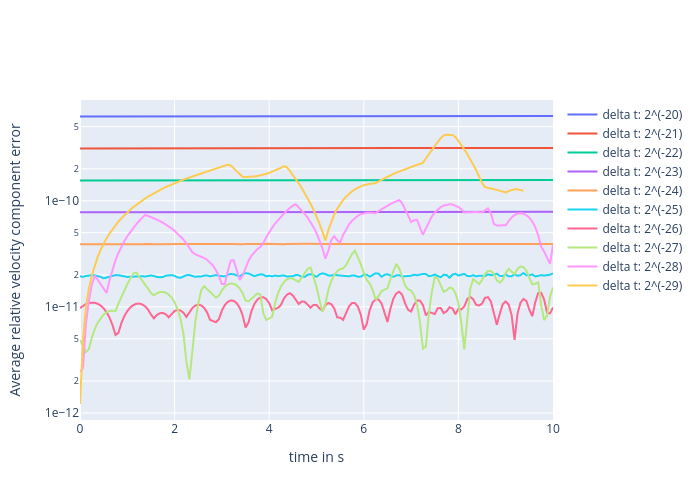
\includegraphics[width=.9\columnwidth]{figures/rel_err_short_2.png}
            \caption[Relative velocity error]{Relative velocity error average of x,y,z components}
            \label{fig:rel_err}
        \end{figure}
        \item Determin \(\Delta t\) required to achieve an error smaller than 1e-8 and 1e-16
        \item Fix run time and compare achievable error
    \end{itemize}

\chapter{Run time analysis}
    \begin{itemize}
        \item Run simulations with heyoka to compare run time
        \item Fix The Error to 1e-8 and 1e-16 and compare run time over a selection of starting value to average out sweet spots for heyokas adaptive time steps
        \item Run Simulations with different amounts of particles and analyze the run time compared to heyokas batch mode.
        \item Profile time spent for calculating the different acceleration components
    \end{itemize}

\chapter{Acceleration component analysis}
    \begin{itemize}
        \item Run simulations with multiple particles covering the domain of relevant satellite orbits and analyze the contributions of the acceleration components with respect to different parameters
        \item Create a Cost/Contribution ratio for the different acceleration components using the profiling data from the run time analysis
    \end{itemize}

\part{Conclusion}
    \begin{itemize}
        \item
        \item
        \item
    \end{itemize}

\appendix
\part{Appendix}

\listoffigures

\listoftables

\bibliographystyle{alpha}
\bibliography{literature}

\end{document}
